\documentclass[12pt, varwidth, border=5mm]{standalone}
\usepackage{tikz}
\usepackage{amsmath}
% Underlining package
\usepackage{ulem}
\usetikzlibrary{calc}
\usetikzlibrary{angles,quotes}
% \usepackage[a4paper, portrait, margin=1cm]{geometry}

\begin{document}
\section*{ }
    \begin{minipage}{0.55\textwidth}
  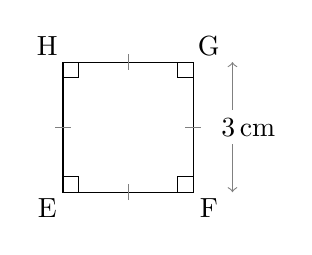
\begin{tikzpicture}[scale=1.0, baseline=(current bounding box.north)]
    \begin{scope}[rotate=0]
        % Draw square
        \draw (0,0) coordinate (E) --
              ++(1.652,0) coordinate (F) --
              ++(0,1.652) coordinate (G) --
              ++(-1.652,0) coordinate (H) -- cycle;

        % Right angle markers
        \foreach \p/\q/\r in {H/E/F,E/F/G,F/G/H,G/H/E} {
            \pic [draw, -, angle radius=0.2cm] {right angle=\p--\q--\r};
        }

        % Vertex LABELS
        % Labels relative to shape geometry
        \node at ($(E)+(-0.2,-0.2)$) {E};
        \node at ($(F)+(0.2,-0.2)$) {F};
        \node at ($(G)+(0.2,0.2)$) {G};
        \node at ($(H)+(-0.2,0.2)$) {H};

        % Tick marks across horizontal sides
        \draw[thin, gray]
            ($(E)!0.5!(F) + (0,-0.10)$) --
            ($(E)!0.5!(F) + (0,0.10)$);

        \draw[thin, gray]
            ($(H)!0.5!(G) + (0,-0.10)$) --
            ($(H)!0.5!(G) + (0,0.10)$);

        % Tick marks across vertical sides
        \draw[thin, gray]
            ($(F)!0.5!(G) + (-0.10,0)$) --
            ($(F)!0.5!(G) + (0.10,0)$);

        \draw[thin, gray]
            ($(E)!0.5!(H) + (-0.10,0)$) --
            ($(E)!0.5!(H) + (0.10,0)$);

        % dotted/dashed arrows shifted away from edges
        % % Vertical side (B-C), shifted right
        \draw[<->, gray]
            ($(F) + (0.50cm,0)$) -- ($(G) + (0.50cm,0)$)
            node[black, midway, fill=white, xshift=2mm, inner sep=3pt] {3\,\text{cm} };

    \end{scope}
\end{tikzpicture}
\end{minipage}%
\hfill
\begin{minipage}{.4\textwidth}
  \begin{align*}
  \text{Perimeter} &= 4l \\
  \text{Perimeter} &= \dotuline{~~~~~~~} \times \dotuline{~~~~~~~} \,\text{\dotuline{~~~~~~~}} \\
  \text{Perimeter} &= \dotuline{~~~~~~~} \,\text{\dotuline{~~~~~~~}}
  \end{align*}
\end{minipage}

\end{document}
